\subsection{Skill Forgetting and Recovery}
Sequential training strongly affects earlier instructions (Fig.~\ref{fig:retention}). Reaching success falls from a mean of 64.1\% to 5.3\% after placement RL, and to 1.8\% after placement-only imitation.

In a separate retention experiment, balanced self-imitation raises reaching from 8.0\% to 31.1\%. Plate placement changes from 50.0\% to 52.3\%, and bowl placement from 23.05\% to 27.65\%. The bank combines earlier reaching successes with current placement successes. Each skill is evaluated under its own fixed reset protocol; placement skill tests can begin with a held object.

\begin{figure*}[!t]
\centering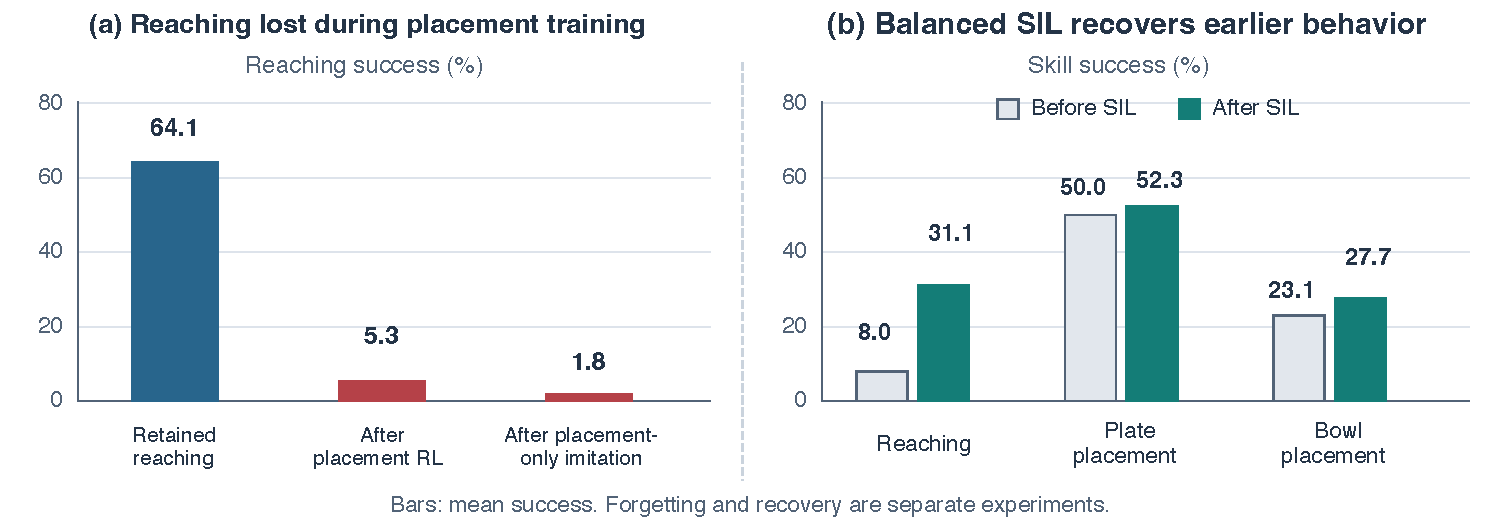
\includegraphics[width=\textwidth]{figures/skill_retention.pdf}
\caption{Forgetting and recovery across instructions. Left: reaching after placement RL and placement-only imitation, with three evaluation rounds per condition. Right: before and after balanced self-imitation, with three reaching rounds and two placement rounds. Bars show means. The panels are separate experiments.}
\label{fig:retention}
\end{figure*}

Recovery is partial, but it preserves placement while improving reaching. Placement-only imitation does not provide this balance. These skill-level results do not isolate the contribution of self-imitation to final full-task success.
